\documentclass{school-22.101-notes}
\date{November 21, 2011}

\begin{document}
\maketitle

%%%%%%%%%%%%% Beta Decay %%%%%%%%%%%%%%%%%
\topic{Beta Decay}
\begin{itemize}
\item Unlike alpha decay where we assume alpha particle is pre-formed, beta decay is more like transformation (from neutrons to protons, protons to neutrons), or say the creations \& annihilation of electrons and positrons, unlike the `preformed alpha-particle in daughter nuclei' theory\footnote{See Krane 9.1-9.4 for details.}. 
\item Energy, linear momentum, angular momentum, parity $\Pi$ are not conserved in the initial observations.
\item Accompanying the emission of electrons and positrons, we introduce neutrinos ($\nu, \bar{\nu}$), a weakly interacting with matter, to conserve terms. Although parity is still not conserved though -- modern unified theory of electro-weak interaction is used to explain that.  
\end{itemize}
\subtopic{Conservation of Energy \& Momentum, First Attempt}
We start with the simpliest form of beta decay: \ce{n \to p + \beta}. Assume neutron is at rest.
\begin{align}
m_n c^2 &= m_p c^2 + m_{\alpha} c^2 + T_{\beta} + T_p &  Q &= (m_n -m_p - m_{\alpha}) c^2 = T_{\beta} + T_p \\
|P_p| &= |P_{\beta}| & T_{\beta} &\mbox{ should be a fixed value like for }T_{\alpha}
\end{align}

\subtopic{Reality Check, Introduce Neutrino}
\begin{figure}
    \centering
    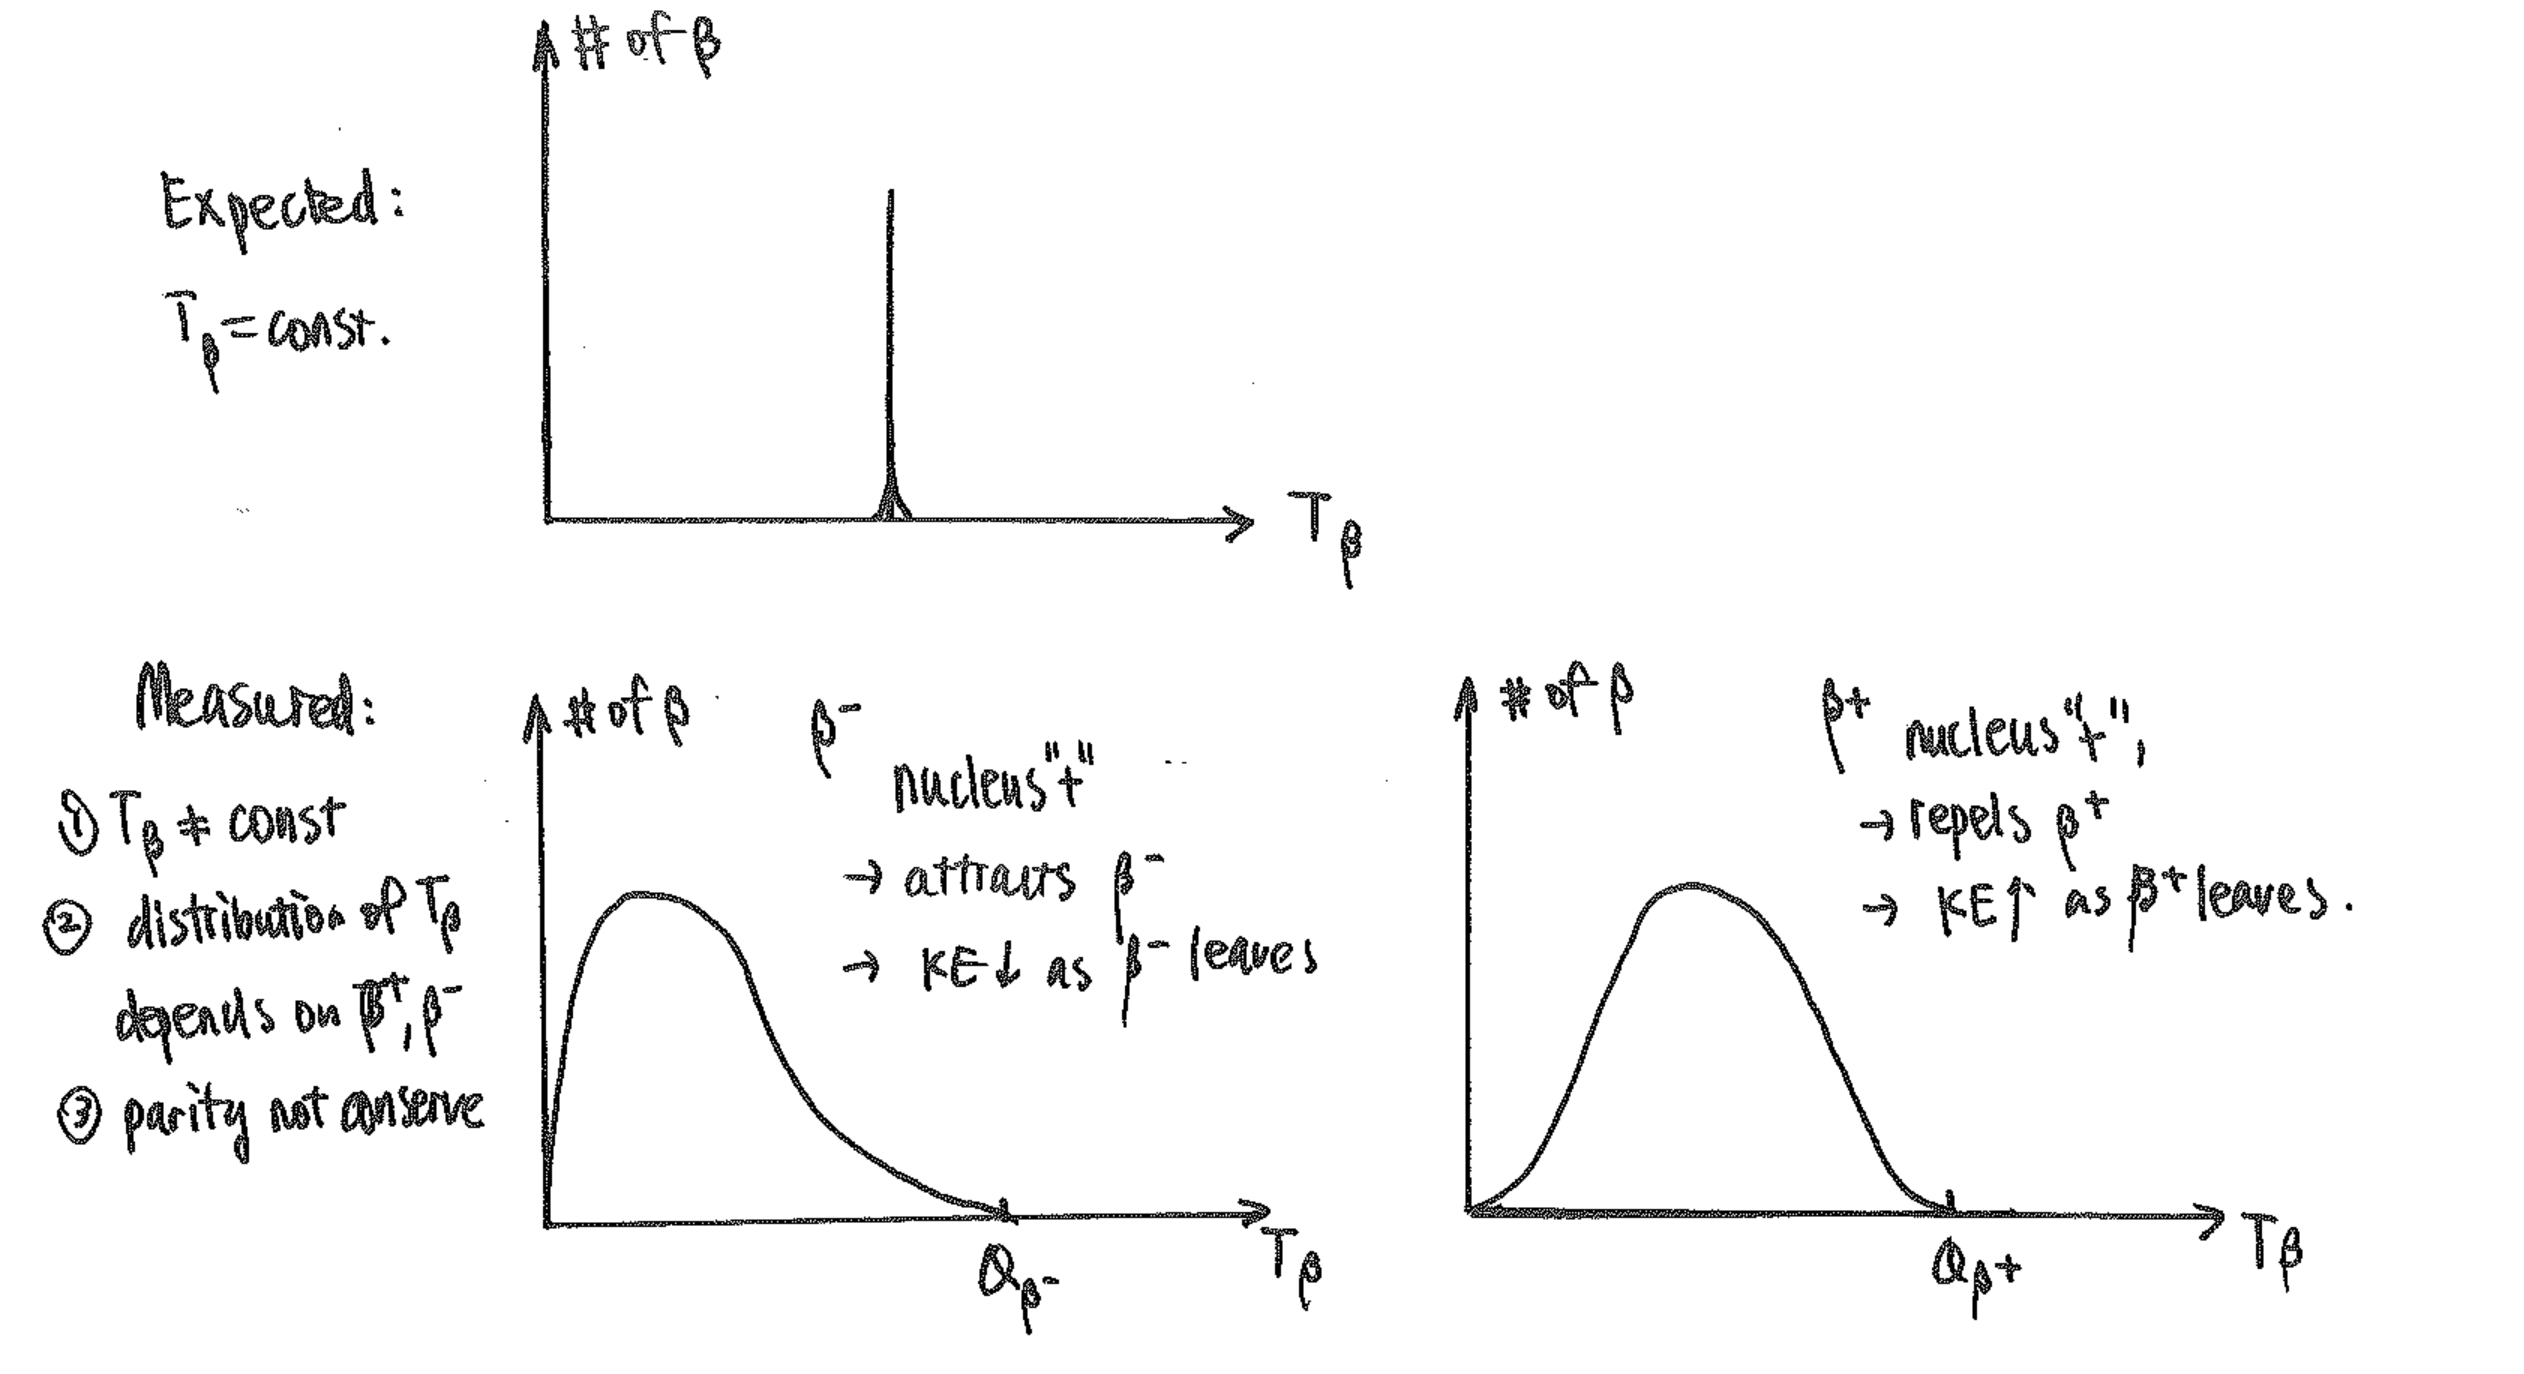
\includegraphics[width=6in]{images/rd/beta-vs-T.png}
    \caption{Expected vs Measured Number of Beta Decays\label{beta-vs-T}}
\end{figure}
\begin{enumerate}
\item $T_{\beta} \neq$ constant. It is a spectrum distribution. After introducing nutrinos, $Q_{\beta}$: $T_{\beta} + T_{\bar{\nu}} = Q_{\beta}, T_{\beta}^{\mathrm{max}} = Q_{\beta}, \expect{T_{\beta}} < Q_{\beta}$. 
\item Electrostatic results: 
    \begin{enumerate}
    \item $\beta^+$: nucleus repels $\beta^+$, KE $\up$.
    \item $\beta^-$: nucleus attracts $\beta^-$, KE $\down$. 
    \end{enumerate}
\item Parity does not conserve yet: \ce{^3H \to \ce{^3He} + e^-}, $\frac{1}{2} \neq 0 \mbox{ or } 1$ (from $ \frac{1}{2} + \frac{1}{2}$).
\item $N(T_{\beta}) \Rightarrow \lambda_{\beta} (E_f)$: number of beta particles is depend on energy; hence decay constant for beta decay is dependent on energy as well.
\end{enumerate}
To explain point 1 \& 3, we introduce neutrino, which are:
\begin{itemize}
\item charge  =0, neutral particles;
\item spin = $\frac{1}{2}$;
\item mass $< \frac{1}{2000} m_e \sim 0 $
\item penetrate easily.  
\item neutrino $\nu$ accompanies $\beta^+$, antineutrino $\bar{\nu}$ accompanies $\beta^-$.
\end{itemize}
The updated beta decays are: 

\ce{^A_Z X_N ->[\beta^-] ^Z_{Z+1} X_{N-1} + e^- + \bar{\nu}};

\ce{^A_Z X_N ->[\beta^+] ^Z_{Z-1} X_{N+1} + e^+ + \nu};

\ce{e + p ->[e.c.] n + \nu}.

The energetics associated with these updated beta decays are (notice $m_n$ is nucleus mass, m is atomic mass; keep in mind $Q>0$ is the criterion for a decay to happen):
\begin{align}
Q_{\beta^-} &= \left[ m_n (\ce{^A_Z X_N}) - m_n (\ce{^A_{Z+1} X_{N+1}}) - m_e \right] c^2 = \left[ m (\ce{^A_Z X_N}) - m (\ce{^A_{Z+1} X_{N}}) \right] c^2 \\
Q_{\beta^+} &= \left[ m (\ce{^A_Z X_N}) - m (\ce{^A_{Z-1} X_{N}}) - 2m_e \right] c^2 \\
Q_{\epsilon} &= \left[ m (\ce{^A_Z X_N}) - m (\ce{^A_{Z+1} X_{N+1}}) \right] c^2 - B_n 
\end{align}

\end{document}
